% !TeX root = Bachelorarbeit.tex
\chapter{Organisation}
\label{Organisation}
\section{Workflow}
Der bereits im Praxisprojekt \cite{PraxBerJoSc} etablierte Workflow wurde zu einem großen Teil übernommen. 
Tägliche Treffen jedoch entfielen, da der Autor nicht in einem Team arbeitete.

Anforderungen an die Software wurden als Stories in dem \glqq Issues \grqq-Tab des verwendeten GitHub Repositories als User Story eingetragen. Abbildung  \ref{fig:EinzelStory} zeigt eine solche Story.


\begin{figure}[htbp] 
  \centering
     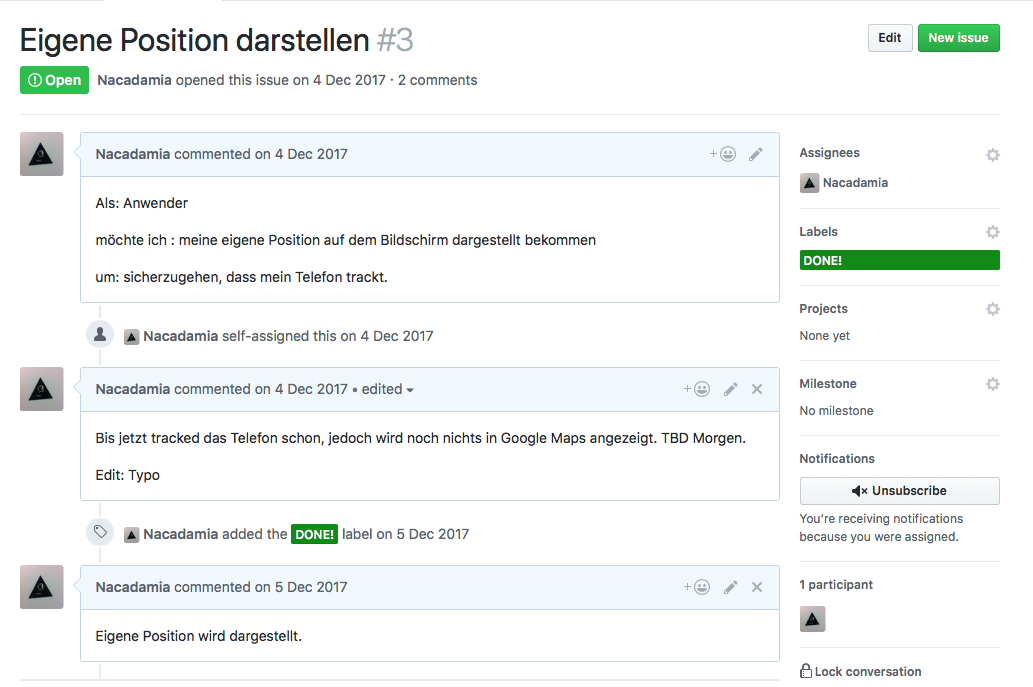
\includegraphics[width=0.8\textwidth]{images/EinzelStory.png} 
  \caption{Einzelne Story im Issues-Tab des \emph{Bustracker} Repository}
  \label{fig:EinzelStory}
\end{figure}

Es wurden Stories aus dem in Abbildung \ref{fig:IssuesTab} gezeigten IssusesTab gewählt. Nach Abschluss einer Story bzw. Implementierung eines Features, wurde diese mit dem Label \glqq Done\grqq{} versehen. Nach positiver Abnahme wurde die Story dann auf \glqq closed\grqq{} gesetzt und somit geschlossen.

\begin{figure}[htbp] 
  \centering
     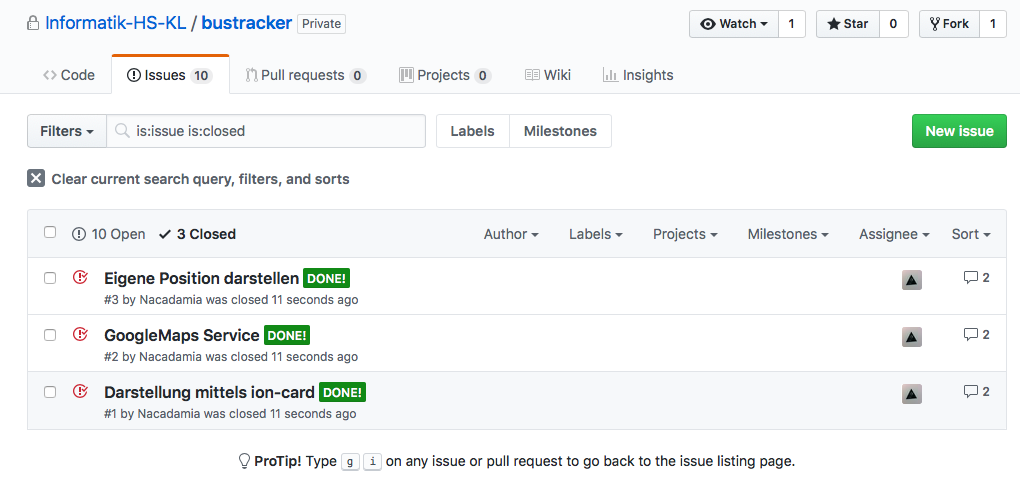
\includegraphics[width=0.8\textwidth]{images/issues_tab.png} 
  \caption{Issues-Tab des Repository}
  \label{fig:IssuesTab}
\end{figure}

Um die Positionsdaten zu erfassen und im Anschluß wieder zu verteilen wird eine Datenbank benötigt. Die gewählte Datenbank ist eine sogenannte MariaDB \cite{MariaDBDoku}.
Die gewählte Datenbankstruktur und die benötigten Daten sind in Abb. \ref{fig:ERD} dargestellt.

\begin{figure}[htbp] 
	\centering
	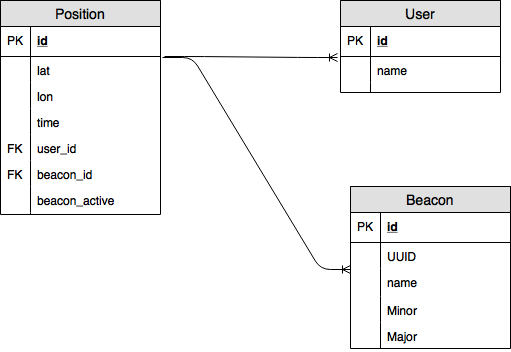
\includegraphics[width=0.8\textwidth]{images/ERDiagramm_bustracker.png} 
	\caption{ER-Diagramm der Bustracker Datenbank}
	\label{fig:ERD}
\end{figure}

 Die API-Entwicklung wurde extern durchgeführt. Die entstandene REST-API ist in \cite{btapidoku} beschrieben. 
\section{Ablauf}

Zu Beginn der Arbeit wurden die benötigten Funktionalitäten für \emph{Bustracker} identifiziert. Diese wären zum einen die Möglichkeiten zur Positionsbestimmung \gls{gls:css} und iBeacons und zum anderen die Anzeige der zuvor bestimmten Position. Dies wurde mittels der Brainstorming Technik durchgeführt. (Abbildung \ref{fig:Brainstorming}).

Für den Prototypen kommt hier aufgrund der einfachen Implementierung und umfangreicher \glspl{gls:API}  GoogleMaps in Frage. Um den Zustand der App speichern zu können bot sich der Zugriff auf den Festspeicher des jeweiligen Endgerätes an.  Um dem eigentlichen Zweck, die Mitteilung der eigenen Position an ein anderes Endgerät zu übertragen, zu entsprechen, müssen die Daten weitergeleitet werden.  Dazu wird bei \emph{Bustracker} eine \nameref{REST} - \nameref{API} eingesetzt.  

\begin{figure}[htbp] 
  \centering
     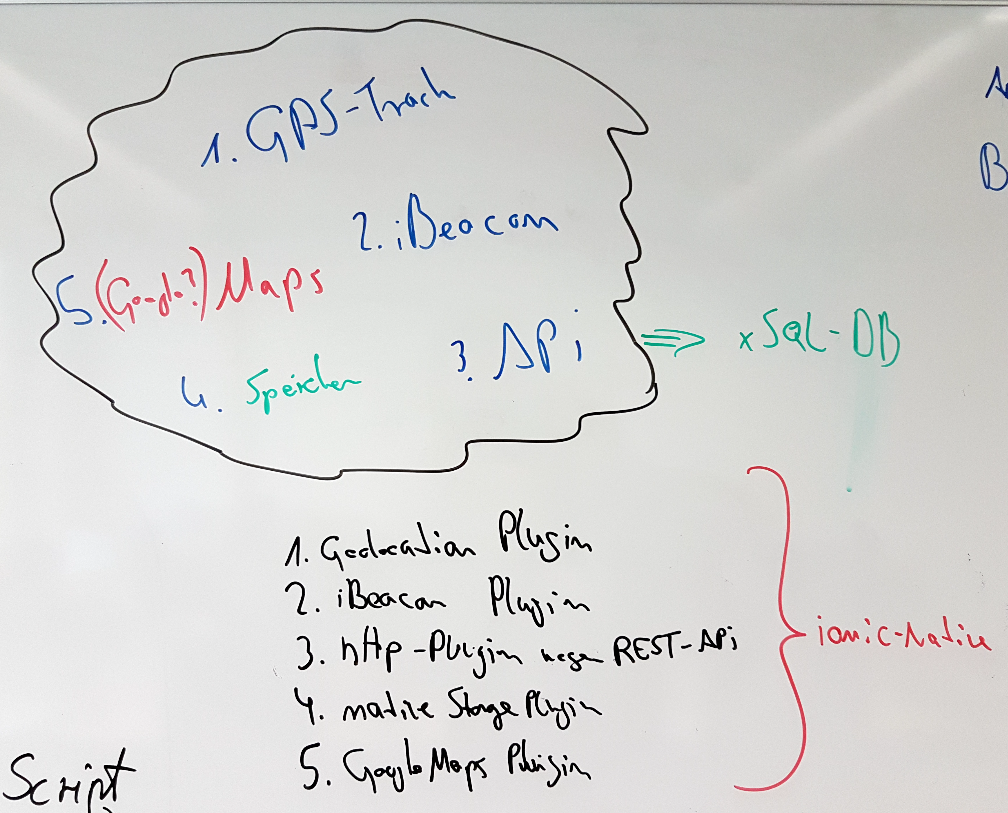
\includegraphics[width=0.8\textwidth]{images/brainstorming.png} 
  \caption{Ergebnis des Brainstormings}
  \label{fig:Brainstorming}
\end{figure}

\nameref{ionic} bietet eine Reihe von Plugins an, mit denen die native Hardware des Gerätes plattformunabhängig angesprochen wird. Alle Funktionen können mittels solcher \emph{native Plugins} abgebildet werden. Zur konkreten Implementierung siehe Kapitel \nameref{Backend}.

Im Anschluss an diesen Teil erfolgte die Implementierung von Teilfunktionen um mehr über das Verhalten der einzelnen Plugins herauszufinden. Parallel wurde das Aussehen des \gls{gls:gui} in sogenannten Scribbles skizziert. Ein Beispiel ist das Scribble der WatchPage in Abbildung \ref{fig:scribble}. 

\begin{figure}[htbp] 
  \centering
     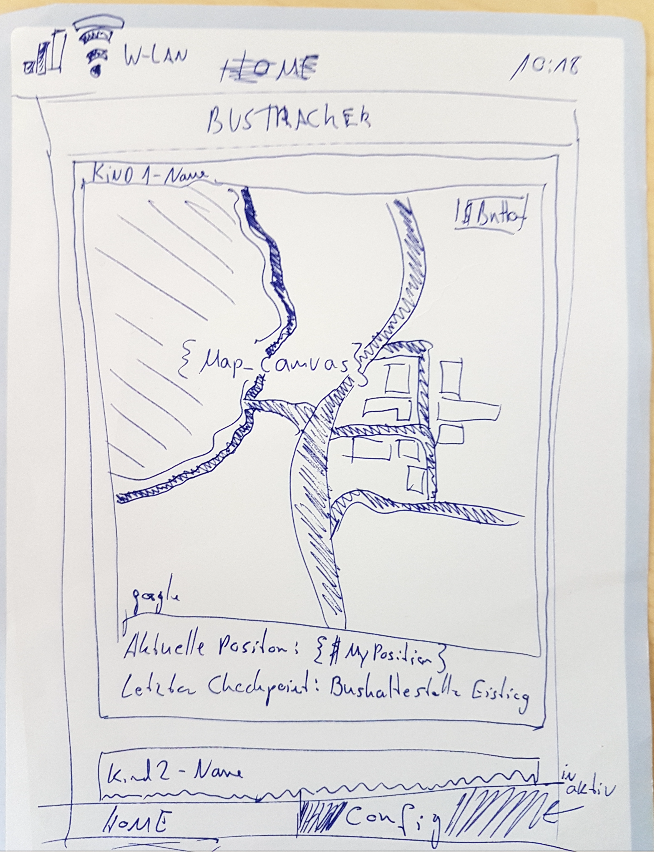
\includegraphics[width=0.6\textwidth]{images/scribble.png} 
  \caption{Scribble der WatchPage}
  \label{fig:scribble}
\end{figure}

Nach dem Vorbild der Scribbles wurden die Seiten gestaltet. Im Anschluss daran wurden die Komponenten ausgewählt, um die geplanten Funktionalitäten bereitzustellen. Diese Komponenten wurden eingebunden und damit der gewünschte Funktionsumfang geschaffen. Nachdem die Komponenten erfolgreich getestet wurden, erfolgte die externe Anbindung an die \gls{gls:API}.
Am Ende wurde die Benutzeroberfläche einheitlich gestaltet.

